\section{Experiment}
\label{sec:exp}

\subsection{Experimental Setup}

\subsubsection{Datasets}
\label{sec:setup_data}
We evaluate on two driving benchmarks, and on each the router is trained only on
still detection images and tested on video, with no tracking or temporal
supervision at any stage.

\noindent\emph{KITTI.} The router is trained on KITTI Detection~\cite{geiger2012kitti}
(80:20 split, $5985/1496$ train/val images) and evaluated on the KITTI
Multi-Object Tracking set ($21$ videos, $8008$ frames), scoring the
\texttt{car}/\texttt{pedestrian}/\texttt{cyclist} classes. Frames are processed at
$384\times1248$.

\noindent\emph{BDD100K.} As a cross-dataset test, the router is trained on the
BDD100K~\cite{yu2020bdd} detection images ($70$k train / $10$k val, $10$ classes)
and evaluated on the BDD100K MOT validation videos
($200$ sequences labeled at $5$\,fps); routing and scoring run at the labeled $5$\,fps
cadence, and we score the $8$ movable classes the MOT split annotates
(\texttt{pedestrian}, \texttt{rider}, \texttt{car}, \texttt{bus}, \texttt{truck},
\texttt{bicycle}, \texttt{motorcycle}, \texttt{train}). The MOT labels provide no
tracks for the static \texttt{traffic\,light}/\texttt{sign} classes that the
$10$-class detector also predicts, so we exclude those two classes at scoring time
to avoid penalizing every prediction as a false positive; this aligns the evaluated
taxonomy with the labels and is applied identically to all strategies. Frames are
processed at $720\times1280$, and the underlying AnyDepth detector is the
BDD-finetuned model, likewise kept frozen.


\subsubsection{Video Evaluation Protocol}
To compare every routing strategy on an identical detection pool, we run both the base and the super path on every frame and cache their detections; a strategy then differs only in which path's detections it keeps for that frame and in how it makes that choice. 
This isolates the routing decision from detector variance, so all strategies (ours and the baselines) are scored in a single pass over the video and are directly comparable. 
Routing is causal and recursive: the decision for frame $t$ is made from features produced by the path that was actually executed on frame $t{-}1$ (the first frame defaults to the base path), so no extra forward is needed to decide. 
Accuracy is reported as AP@.50 and AP@[.50:.95] obtained by matching the kept detections to the KITTI-tracking labels over all frames pooled.
Per-frame computation is obtained from a precomputed lookup of the super/base FLOPs and aggregated by the realized SUPER-usage rate. 
On-device latency and energy are measured per frame on the target GPU with device synchronization and board-power sampling, after a warm-up phase; crucially, the router's own forward is timed and charged to the routing strategy, so the reported latency, FPS, and energy
include the router overhead.

This evaluation protocol mirrors the deployment routing loop
(Algorithm~\ref{alg:routing}), except that here both paths are cached every frame
so all strategies share one detection pool; the latency-budget tracking experiment
(Sec.~\ref{sec:results_budget}) likewise replays the PI controller of
Algorithm~\ref{alg:budget}.


\subsubsection{Implementation Details}
\label{sec:setup_impl}
The router is trained for 300 epochs (batch 256, Adam, lr $10^{-3}$) over seeds 0--4
and reported as mean$\pm$std. 
The detector is frozen; only the router is updated, so
each epoch is a cheap pass over the cached features. 
Detection uses confidence threshold $0.25$ and NMS IoU $0.7$.


 
\subsubsection{Evaluation Metrics}
\label{sec:setup_metrics}
%% TODO
% AP@[.50:.95], AP@.50, SUPER usage %, GFLOPs/frame.
% On-device: latency (ms), FPS, energy (mJ), and deltas vs. super-only.
% Router overhead: #params, FLOPs.
We report AP@[.50:.95] and AP@.50, the SUPER-path usage rate, and GFLOPs/frame.
On-device measurements (latency, FPS, energy) include the router forward and are
reported against the super-only reference. Router cost is given as \#params and
FLOPs (Table~\ref{tab:overhead}).
 
%% =====================================================================
\subsection{Results}
\label{sec:results}
 
\subsubsection{Main Result: Pareto Dominance}
\label{sec:results_main}

\begin{figure*}[t]
\centering
\begin{minipage}[t]{0.49\textwidth}
\centering

\includegraphics[width=\linewidth]{fig_main_ap5095.pdf}
\vspace{2pt}
{\small (a) KITTI}
\end{minipage}\hfill
\begin{minipage}[t]{0.49\textwidth}
\centering

\includegraphics[width=\linewidth]{fig_main_bdd_ap5095.pdf}
\vspace{2pt}
{\small (b) BDD100K}
\end{minipage}
\caption{Depth routing (AP@[.50:.95] vs.\ SUPER usage): the proposed
advantage-regression router (threshold sweep; TinyConv head, $2\times2$ grid) vs.
random, luminance, and edge-density baselines, on (a) KITTI-tracking and
(b) BDD100K MOT (cross-dataset, router trained only on still images). The single
trained router traces a
continuous Pareto front that dominates all baselines, most strongly in the
low-budget (low SUPER-usage) region.}
\label{fig:main}
\end{figure*}


\begin{table*}[t]
\caption{Efficiency across every threshold $\tau$ in Fig.~\ref{fig:main} (TinyConv
router; latency, FPS, energy on an RTX~3090, including the router forward). AP is
AP@[.50:.95] (\%). \textsc{a-base}/\textsc{a-super} are the static single-path
configurations (the endpoints of the curve in Fig.~\ref{fig:main}; $\tau\!\to\!\pm\infty$). Absolute
latency/energy are not comparable across datasets (BDD100K uses a larger input and
$\approx2\times$ the GFLOPs); only the within-dataset trade-off is meaningful.}
\label{tab:device}
\small
\setlength{\tabcolsep}{2.5pt}
\centering
\begin{minipage}[t]{0.49\textwidth}
\centering
{\small (a) KITTI}\\[2pt]
\footnotesize
\begin{tabular}{lrrrrrr}
\toprule
$\tau$ & SUPER\% & GFLOPs & AP & Latency (ms) & FPS & Energy (mJ)\\
\midrule
\textsc{always-base} & 0.0 & 16.87 & 39.3 & 13.35 & 74.9 & 2139\\
$+0.70$ & 1.5 & 17.01 & 39.5 & 13.80 & 72.5 & 2213\\
$+0.50$ & 3.8 & 17.23 & 39.8 & 13.96 & 71.6 & 2239\\
$+0.40$ & 7.4 & 17.57 & 40.2 & 14.24 & 70.2 & 2283\\
$+0.30$ & 13.9 & 18.18 & 40.6 & 14.73 & 67.9 & 2362\\
$+0.20$ & 26.7 & 19.39 & 41.0 & 15.69 & 63.7 & 2515\\
$+0.10$ & 52.2 & 21.80 & 41.4 & 17.61 & 56.8 & 2823\\
$+0.00$ & 82.3 & 24.64 & 41.5 & 19.87 & 50.3 & 3185\\
$-0.10$ & 96.1 & 25.93 & 41.5 & 20.91 & 47.8 & 3351\\
$-0.20$ & 99.0 & 26.21 & 41.5 & 21.13 & 47.3 & 3386\\
$-0.40$ & 99.6 & 26.27 & 41.5 & 21.17 & 47.2 & 3394\\
\textsc{always-super} & 100.0 & 26.30 & 41.5 & 20.87 & 47.9 & 3343\\
\bottomrule
\end{tabular}
\end{minipage}\hfill
\begin{minipage}[t]{0.49\textwidth}
\centering
{\small (b) BDD100K}\\[2pt]
\footnotesize
\begin{tabular}{lrrrrrr}
\toprule
$\tau$ & SUPER\% & GFLOPs & AP & Latency (ms) & FPS & Energy (mJ)\\
\midrule
\textsc{always-base} & 0.0 & 33.18 & 21.3 & 24.76 & 40.4 & 8389\\
$+0.069$ & 15.4 & 36.03 & 21.7 & 27.25 & 36.7 & 9145\\
$+0.057$ & 30.2 & 38.78 & 22.0 & 29.39 & 34.0 & 9872\\
$+0.051$ & 42.4 & 41.04 & 22.2 & 31.14 & 32.1 & 10468\\
$+0.046$ & 53.4 & 43.08 & 22.2 & 32.72 & 30.6 & 11008\\
$+0.042$ & 62.0 & 44.67 & 22.3 & 33.96 & 29.4 & 11427\\
$+0.038$ & 69.2 & 46.00 & 22.3 & 34.99 & 28.6 & 11779\\
$+0.034$ & 75.8 & 47.23 & 22.4 & 35.95 & 27.8 & 12104\\
$+0.030$ & 82.0 & 48.37 & 22.4 & 36.84 & 27.1 & 12407\\
$+0.023$ & 88.9 & 49.66 & 22.4 & 37.83 & 26.4 & 12746\\
$-0.027$ & 99.4 & 51.62 & 22.5 & 39.35 & 25.4 & 13263\\
\textsc{always-super} & 100.0 & 51.72 & 22.5 & 39.16 & 25.5 & 13289\\
\bottomrule
\end{tabular}
\end{minipage}
\end{table*}

We compare our advantage-regression router against four routing strategies that
share the same frozen detector and differ only in the per-frame signal used to
choose a path: random routing, luminance- and edge-density--based routing, and
confidence routing (the mean of the top-$20$ box scores, or of the scores
$\ge0.1$, on the previous frame); each is swept over its decision threshold to
trace a curve. Fig.~\ref{fig:main} shows that on \emph{both} datasets the single
trained router traces a continuous Pareto front that dominates every baseline across
the operating range, while the baselines reach super-only accuracy only near
$100\%$ SUPER usage (i.e., with no savings). On KITTI (Fig.~\ref{fig:main}(a)) the router holds
AP@[.50:.95] within $0.1$ point of the super-only ceiling ($41.4$ vs.\ $41.5$) while
routing only $52\%$ of frames to the deep path, i.e.\ at $21.8$ rather than $26.3$
GFLOPs/frame ($-17\%$ compute); pushing to $27\%$ SUPER usage costs just $0.2$ AP
for a $26\%$ compute reduction, whereas at the same budgets the strongest baseline
still trails the super-only line by $1$--$2$ points. On BDD100K
(Fig.~\ref{fig:main}(b)) the curve has the same shape: at only $30\%$ SUPER usage
the router already recovers the bulk of the deep-path gain ($22.0$ vs.\ $22.5$
AP@[.50:.95]) at $25\%$ less compute. On both, the margin over the baselines is
widest in the low-budget (low SUPER-usage) region, where choosing \emph{which}
frames deserve the deep path matters most. Notably, BDD100K is a cross-dataset
test---the router is trained only on still BDD images with no tracking or temporal
supervision---yet it transfers to the MOT video unchanged, confirming that the
formulation is not KITTI-specific.

Table~\ref{tab:device} confirms that these FLOP savings translate into real
on-device gains once the router forward is charged to the budget. At the KITTI
sweet-spot ($\tau{=}{+}0.10$) the $17\%$ compute cut yields $16\%$ lower latency and
energy and $19\%$ higher FPS at no accuracy loss; on BDD100K the $30\%$-SUPER
operating point gives $25\%$ lower latency, $26\%$ lower energy, and $34\%$ higher
FPS. The router overhead (Table~\ref{tab:overhead}) is below $0.002\%$ of the SUPER
path, so the measured savings track the FLOP reduction almost exactly.


\subsubsection{Advantage Regression Quality}
\label{sec:results_calibration}
Fig.~\ref{fig:calibration} relates the router's predicted advantage $\hat{A}$ to
the true per-image loss gap $A$ on the validation set (Pearson $r{=}0.37$). The
correlation is positive but deliberately modest, and this is expected rather than a
weakness: the regression target is a \emph{single-image} loss difference, an
intrinsically noisy quantity (the same scene yields a different gap under small
appearance changes), so no predictor---however expressive---can correlate tightly
with it. What the router must get right is not the exact magnitude but \emph{which}
frames benefit most from the deep path, and the prediction is compressed toward the
mean precisely because it averages out this label noise. The decisive evidence that
the signal is good enough is downstream: thresholding this $\hat{A}$ yields the
continuous, baseline-dominating Pareto front of Fig.~\ref{fig:main} on both
datasets---an operating-point quality that a poorly ordered score could not
produce.
\begin{figure}[t]
\centering
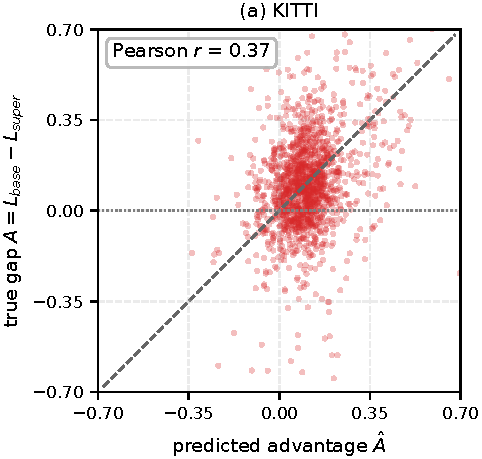
\includegraphics[width=0.7\columnwidth]{fig_calibration.pdf}
\caption{Predicted advantage $\hat{A}$ vs. true loss gap
$A=L_{\mathrm{base}}-L_{\mathrm{super}}$ on the KITTI validation set (5-seed
ensemble). The router orders images by how much the deep path helps.}
\label{fig:calibration}
\end{figure}


\begin{figure}[t]
\centering

\includegraphics[width=0.9\columnwidth]{fig_advantage_dist.pdf}
\caption{Per-image advantage $A=L_{\mathrm{base}}-L_{\mathrm{super}}$ distribution.
BDD100K is concentrated near zero (small base$\to$super gap, $\sigma{=}0.12$),
KITTI is roughly twice as wide ($\sigma{=}0.23$); the smaller, noisier BDD100K gap
is why feature source barely matters and the operating range is spanned by a narrow
$\tau$ band there.}
\label{fig:adv_dist}
\end{figure}

 
\subsubsection{On-Device Efficiency}
\label{sec:results_device}


\begin{table}[t]
\caption{Router overhead (per frame, batch $1$). Both routers add negligible cost
relative to the SUPER path ($26.30$ GFLOPs).}
\label{tab:overhead}
\centering
\begin{tabular}{lrrr}
\toprule
Router & \#Params & GFLOPs & \% of SUPER\\
\midrule
GAP-MLP & 60{,}241 & $1.17\times10^{-4}$ & $0.0004$\\
TinyConv ($2\times2$) & 60{,}881 & $4.17\times10^{-4}$ & $0.0015$\\
TinyConv ($4\times4$) & 60{,}881 & $1.61\times10^{-3}$ & $0.0060$\\
\bottomrule
\end{tabular}
\end{table}

\subsubsection{Runtime Latency-Budget Tracking}
\label{sec:results_budget}
The threshold $\tau$ exposes the operating point as a single scalar knob, so the
detector can be \emph{steered at runtime} to follow a time-varying latency budget
$L^\star(t)$ (e.g.\ a thermal- or battery-driven schedule) without any retraining.
We close a simple control loop around $\tau$: a PI controller compares the target
to an exponential moving average of the realized per-frame latency and nudges
$\tau$ to cancel the error (lowering $\tau$ admits more SUPER frames, raising
latency; raising it does the opposite). Because per-frame cost is memoryless, we
replay the cached per-frame advantages and the measured path latencies to evaluate
the loop. Fig.~\ref{fig:budget} shows that the realized latency tracks both a
step and a sawtooth budget tightly (mean abs.\ error $0.21$ and $0.23$\,ms) while
detection accuracy is held (AP@[.50:.95] $\approx 44.9$). A single trained router
thus turns the continuous Pareto front into a runtime-adjustable budget the system
can steer frame-by-frame.

\begin{figure*}[t]
\centering
\includegraphics[width=\linewidth]{fig_latency_budget.pdf}
\caption{Runtime latency-budget tracking on KITTI-tracking. A PI controller
adjusts the router threshold $\tau$ each frame so the realized per-frame latency
(moving average, red) follows a time-varying target $L^\star(t)$ (black), for a
step (left) and a sawtooth (right) budget; tracking error is $\approx0.2$\,ms.
Latency uses the measured RTX-3090 path anchors (Table~\ref{tab:device}a).}
\label{fig:budget}
\end{figure*}

%% =====================================================================
\subsection{Ablation Studies}
\label{sec:ablation}
 
\subsubsection{Input Feature Level: Backbone vs. Neck vs. Both}
\label{sec:abl_feature}

\begin{figure}[t]
\centering

\includegraphics[width=0.9\columnwidth]{fig_abl_feat_ap5095.pdf}
\caption{Feature ablation (AP@.50:.95): feature source (backbone/neck/both).}
\label{fig:abl_feat_source}
\end{figure}

We compare three feature sources for the router on both datasets: the backbone
pyramid features (input-level representations, before the detection neck), the neck
features (prediction-level representations, immediately before the heads), and their
concatenation. On KITTI backbone features win and adding the neck does not help
(backbone $>$ both $>$ neck; Fig.~\ref{fig:abl_feat_source}), and
Table~\ref{tab:feat_cross} shows the same conclusion holds on BDD100K, so we adopt a
single backbone-only router throughout.

The two feature sources answer different questions. 
Neck features encode \emph{what the detector currently predicts} under the executed
path; they are informative about confidence on \emph{that} path, but the quantity
we need is \emph{counterfactual}---how much the \emph{other}, deeper path would
improve the result. That gap is largely determined by raw scene properties (clutter,
object scale, lighting) that are most cleanly exposed in the input-level backbone
features and are partially washed out by the time the signal reaches the
prediction-level neck. Concatenating the neck therefore adds variance without adding
discriminative signal, and dilutes the clean backbone cue. This is the same lesson
that lets purely pixel-level signals (edge density, luminance) route
well~\cite{pixels2027}: the benefit of going deep is written into the image content
itself, so input-level features are the right place to read it---\emph{pixels know
when to go deep}.

Quantitatively (Table~\ref{tab:feat_cross}) the ordering is
\emph{dataset-dependent in magnitude but not in conclusion}: on KITTI backbone
features win clearly (a $0.42$-point AUC margin over neck, $\approx5\times$ the
seed std), whereas on BDD100K all three sources are statistically
indistinguishable ($<\!1$ std apart). The difference is explained by the routing
headroom: the BASE$\to$SUPER accuracy gap is only $\approx1.2$ points on BDD100K
versus $\approx2.2$ on KITTI, and the per-image advantage is correspondingly
smaller and noisier---its distribution is concentrated near zero on BDD100K
($\sigma{=}0.12$) and roughly twice as wide on KITTI ($\sigma{=}0.23$;
Fig.~\ref{fig:adv_dist}), which is also why the useful $\tau$ band is narrow on
BDD100K and broad on KITTI (Table~\ref{tab:device}). When the exploitable signal is this small, every
reasonable feature source saturates the same low ceiling and the choice of tap can
no longer differentiate; KITTI, with more exploitable structure, rewards the
cleaner input-level cue. Either way backbone-only is \emph{best-or-tied on both
datasets} and is also the cheapest (no neck tap, smallest router), which is why we
make it the single consistent design.

\begin{table}[t]
\caption{Feature-source comparison across datasets: AUC of the AP@[.50:.95]-vs-SUPER
usage curve (percent, mean$\pm$std over 5 seeds). Backbone is the best-or-tied
choice on both, motivating a single backbone-only router.}
\label{tab:feat_cross}
\centering
\small
\begin{tabular}{lcc}
\toprule
Feature source & KITTI & BDD100K\\
\midrule
backbone (input) & $\mathbf{41.12}\pm0.07$ & $22.12\pm0.02$\\
neck (pred)      & $40.70\pm0.08$ & $22.12\pm0.01$\\
both             & $41.03\pm0.08$ & $\mathbf{22.14}\pm0.01$\\
\bottomrule
\end{tabular}
\end{table}


\subsubsection{Feature Normalization: None vs. BatchNorm1d vs. LayerNorm}
\label{sec:abl_norm}

Fig.~\ref{fig:abl_norm}).
\begin{figure}[t]
\centering
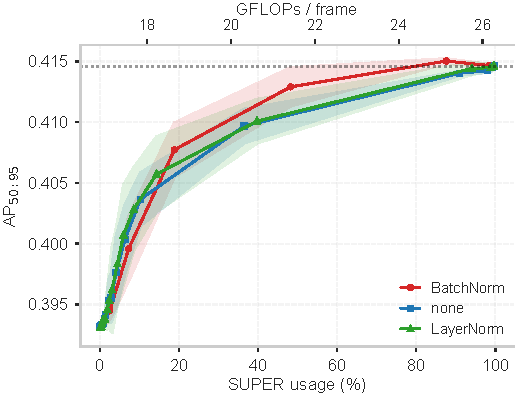
\includegraphics[width=0.9\columnwidth]{fig_abl_norm_ap5095.pdf}
\caption{Feature normalization (none/BN/LN). AP@.50:.95.}
\label{fig:abl_norm}
\end{figure}

We compare no normalization, BatchNorm1d, and LayerNorm on the pooled multi-scale
descriptor (Fig.~\ref{fig:abl_norm}).
The three pyramid levels $\{S_2,S_3,S_4\}$ live at very different activation magnitudes, so without conditioning the largest-scale features dominate the regression and the smaller
scales are effectively ignored. 
The decisive question is \emph{along which axis} the statistics are removed. 
BatchNorm normalizes each feature \emph{across images} in the batch, which equalizes the multi-scale magnitudes while \emph{preserving the relative differences between images}---and it is precisely those between-image differences that encode which frames are hard. 
LayerNorm instead normalizes \emph{within each image} across features, which removes exactly the global ``how active is this whole image'' signal that correlates with difficulty, and can
therefore erase the cue the router needs. 
In short, normalize across images (keep the difficulty ranking), not within an image (which destroys it); BatchNorm is the safe default for this reason, with the additional benefit of well-conditioned multi-scale aggregation.

\subsubsection{Previous-Action Sampling Ratio $p(\mathrm{super})$}
\label{sec:abl_prevaction}
During training we sample the assumed previous action (the path whose features the
router conditions on) as super with probability $p$, sweeping
$p \in \{0.0, 0.25, 0.5, 0.75, 1.0\}$ (Fig.~\ref{fig:abl_prevaction}).
We find $p{=}0.5$ best, with the symmetric extremes tied and worse
($p{=}0.5 > 0.25{=}0.75 > 0.0{=}1.0$).
\begin{figure}[t]
\centering
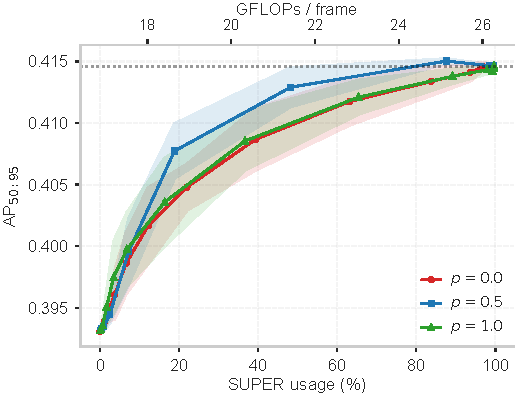
\includegraphics[width=0.9\columnwidth]{fig_abl_prevp_ap5095.pdf}
\caption{Previous-action sampling ratio $p(\mathrm{super})$ during training
(AP@.50:.95). 
% Balanced sampling ($p{=}0.5$) is best; the symmetric extremes ($p{=}0.0$, $p{=}1.0$) are worst.
}
\label{fig:abl_prevaction}
\end{figure}
 
 This is a train/serve distribution-matching effect. 
 At deployment the router must read features produced by \emph{whichever} path ran on
the previous frame---sometimes base, sometimes super---and the same image yields a
slightly different feature map under each path. 
If training only ever shows super-path features ($p{=}1.0$), the router is never calibrated to base-path features and mis-ranks frames whenever the previous frame ran base; $p{=}0.0$ fails symmetrically. 
Training with a balanced $p{=}0.5$ exposes the router to both feature
distributions equally, so its advantage prediction stays calibrated regardless of
which path was executed upstream. 
The takeaway is that the previous action is part of the router's input distribution, and balanced sampling is what makes the causal, per-frame deployment of Sec.~\ref{sec:method_deploy} robust.

 
\subsubsection{Router Design and Grid Resolution}
\label{sec:abl_router}

\begin{figure}[t]
\centering
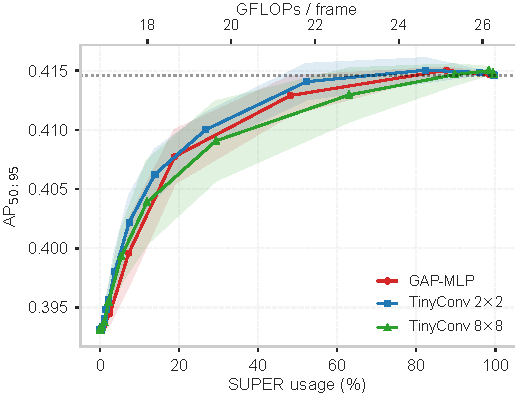
\includegraphics[width=0.9\columnwidth]{fig_abl_router_grid_ap5095.pdf}
\caption{Router design and grid resolution. GAP-MLP is compared with TinyConv
at $2\times2$ and $8\times8$ grids in AP@.50:.95.}
\label{fig:abl_router_grid}
\end{figure}

We compare GAP-MLP with TinyConv at $2{\times}2$ and $8{\times}8$
grids (Fig.~\ref{fig:abl_router_grid}).
TinyConv, which preserves coarse spatial layout, Pareto-dominates GAP-MLP: at $\tau{=}{+}0.10$ it matches the same AP@[.50:.95] using 52\% SUPER versus GAP-MLP's 65\%. Grid resolution beyond $2{\times}2$ does not help, and the $2{\times}2$ TinyConv is the strongest setting.
GAP collapses the whole frame to one vector, so it can only ask ``is this image hard on average?'' 
But difficulty is usually \emph{localized}: a single dense cluster of small objects in one corner of an otherwise empty road is what makes the deep path pay off, and that spatial concentration survives in a $2{\times}2$ grid but is averaged away by global pooling. 
This is why even a tiny amount of retained spatial layout closes a large part of the gap to the deep path.
At the same time, the cue is \emph{coarse}---it is about \emph{where roughly} the
hard content sits, not its fine shape---so a $2{\times}2$ grid already captures it
and a finer $8{\times}8$ grid only adds parameters and variance without
new signal.
The sweet spot is the smallest grid that preserves quadrant-level locality.